%!TEX root =  main.tex
\section{Performance evaluation}
\label{sec:experiments}

In this section, we present the results found for \appname\ with different loads and partitionings and compare them with
\ssmr{}~\cite{bezerra2014ssmr} and \dssmr.
%We are interested in assessing \dssmr{}'s performance with workloads that present different levels of locality.
%By locality, we mean the likelihood that certain groups of data items are accessed together (by the same command).
In Section~\ref{sec:evaluation:setup}, we describe the environment where we conducted our experiments.
In Section~\ref{sec:evaluation:methodology}, we describe how we designed the experiments and our methodology.
In Section~\ref{sec:evaluation:results}, we show the results.

% with strong-locality workloads.
%In Section~\ref{sec:evaluation:weakloc}, we show the results for weak-locality workloads.

%\begin{figure*}
%\begin{minipage}[b]{1\linewidth} % A minipage that covers the whole width of the page
%\centering
%      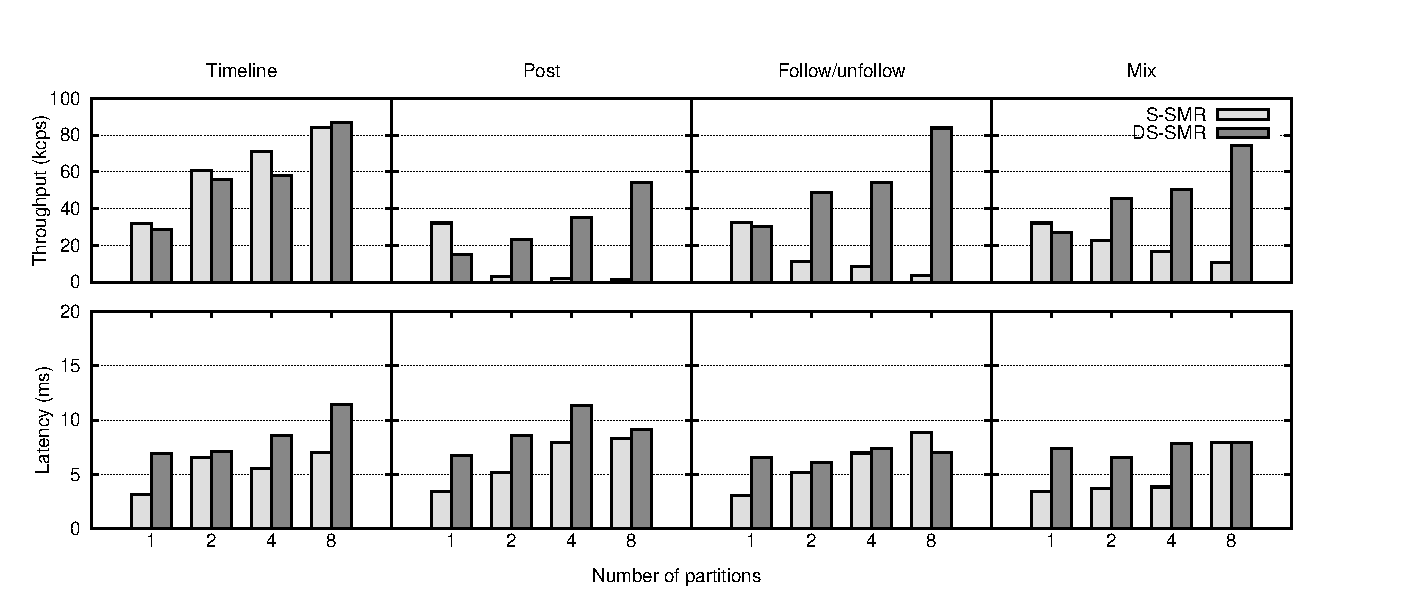
\includegraphics[width=1.08\linewidth]{figures/graphs/strong-locality}
%\end{minipage}
%\caption{Results of \appname\ running with \ssmr\ and \dssmr{}. Throughput is shown in thousands of commands per second (kcps).}
%\label{fig:strongloc}
%\end{figure*}
%\begin{table*}[htp]
%\vspace{10mm}
%\caption{Absolute values of \appname\ running \ssmr\ and \dssmr{}.}
%\centering
%\begin{adjustbox}{max width=\textwidth}
%\begin{tabular}{|l|c|c|c|c|c|c|c|c|c|c|c|c|c|c|c|c|} \hline
%         & \multicolumn{4}{|c|}{Timeline}  &  \multicolumn{4}{|c|}{Post}   &  \multicolumn{4}{|c|}{Follow/unfollow}  &  \multicolumn{4}{|c|}{Mix}    \\ \hline
%         & 1     & 2     & 4     & 8       & 1     & 2     & 4   & 8    & 1     & 2     & 4       & 8           & 1     & 2     & 4     & 8     \\ \hline\hline
%         & \multicolumn{16}{|c|}{Throughput (commands per second)} \\ \hline
%\ssmr\   & 31757 & 60699 & 71274 & 84065   & 32151 & 2884  & 1894  & 1200  & 32541 & 11476 & 8580    & 3371          & 32151 & 22803 & 16822 & 10657 \\ \hline
%\dssmr\  & 28882 & 55925 & 57900 & 86685   & 14874 & 23295 & 35188 & 54250 & 30215 & 48976 & 54025   & 83880         & 27101 & 45686 & 50671 & 74257 \\ \hline\hline
%         & \multicolumn{16}{|c|}{\textbf{Throughput rate = \dssmr\ tput / \ssmr\ tput}} \\ \hline
%         & \textbf{0.91} & \textbf{0.92}  & \textbf{0.81} & \textbf{1.03}     & \textbf{0.46}   & \textbf{8.08}   & \textbf{18.48}  & \textbf{45.00} & \textbf{0.93} & \textbf{4.27} & \textbf{6.30} & \textbf{24.88} & \textbf{0.84} & \textbf{2.00} & \textbf{3.01} & \textbf{6.97} \\ \hline\hline
%         & \multicolumn{16}{|c|}{Latency (milliseconds)} \\ \hline
%\ssmr\   & 3.1 & 6.6 & 5.6 & 7.0  & 3.4 & 5.2  & 7.9  & 8.3  & 3.0  & 5.2  & 7.0  & 8.8  & 3.4  & 3.7  & 3.8  & 7.9  \\ \hline
%\dssmr\  & 6.9 & 7.1 & 8.6 & 11.4 & 6.7 & 8.6  & 11.3 & 9.1  & 6.6  & 6.1  & 7.4  & 7.0  & 7.3  & 6.5  & 7.8  & 7.9  \\ \hline
%\end{tabular}
%\end{adjustbox}
%\label{tbl:results}
%\vspace{10mm}
%\end{table*}%

\subsection{Environment setup and configuration parameters}
\label{sec:evaluation:setup}

We conducted all experiments on a cluster that had two types of nodes: (a) HP SE1102 nodes, equipped with two Intel Xeon L5420 processors running at 2.5 GHz and with 8 GB of main memory, and (b) Dell SC1435 nodes, equipped with two AMD Opteron 2212 processors running at 2.0 GHz and with 4 GB of main memory. The HP nodes were connected to an HP ProCurve 2920-48G gigabit network switch, and the Dell nodes were connected to another, identical switch. Those switches were interconnected by a 20 Gbps link.
All nodes ran CentOS Linux 7.1 with kernel 3.10 and had the OpenJDK Runtime Environment~8 with the \mbox{64-Bit} Server VM (build 25.45-b02).
%We kept the clocks synchronized using NTP in order to measure latency components involving events in different computers.

%For the experiments, we use the following workloads:
%Timeline (composed only of getTimeline requests),
%Post (only post requests),
%Follow/unfollow (50\% of follow requests and 50\% of unfollow), and
%Mix (7.5\% post, 3.75\% follow, 3.75\% unfollow, and 85\% getTimeline).

\subsection{Methodology and goals}
\label{sec:evaluation:methodology}
All weak-locality static graphs were generated using the Holme-Kim model \cite{holme-kim}, with this model we generate
power-law graphs with a clustering coefficient, such graphs, also referred as scale-free, are a good representation
of geometric structures of social networks.

In the experiments, we tested graphs with 10.000 users with a varying percentage of edge-cuts \footnote{An edge is said to be cut if it connects two vertices that are in different partitions}, to get the desired edge-cut
percentage, we run METIS partitioner for each partitioning size. METIS performs well in graphs with less than 10 million nodes, and scales linearly as seen in Figure~\ref{fig:metis_size_time}, with both memory and cpu usage.

\begin{figure}[ht!]
  \centering
    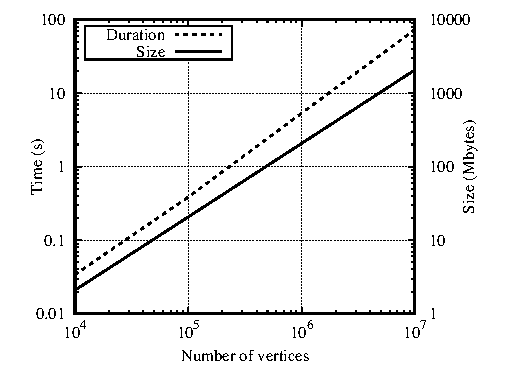
\includegraphics[width=\columnwidth]{figures/metis_size_time}
	\caption{METIS processor and memory usage}
	\label{fig:metis_size_time}
\end{figure}

As explained in the design implementation of \appname\ in Section~\ref{sec:imp:\appname}, we chose to focus our
experiments on the non-trivial case, when a command can go in several partitions. The other commands are linearly
scalable over time, for instance, if a post command is going to be executed 5\% of the time in a graph that have a 10\%
possibility of executing a global command, the actual possibility of executing a global command is 0.05\%.

Since we focus our tests in the post command, we are interested to see what happens when we increase the number of
partitions. With a higher number of partitions we should be able to achieve higher scalability but the amount of edge-cuts
play an important role, the higher the edge-cuts the greater the incentive to degenerate the implementation to a single
partition SMR. To perform how well a system behave in the presence of edge-cuts, we also consider the variation of
edge-cuts. We partition the data in 2, 4 and 8 partitions, for each partitioning we also vary the number of edge-cuts 
in 1\%, 5\% and 10\%, then we put the objects at random initial partitions.
We compare our results with \dssmr\ and \ssmr with a static partitioning produced by METIS.

\subsection{Results}
As we see in the Figure~\ref{fig:varying_edge_cut}, all the techniques perform similar on tests with strong locality, that is
expected because there are no cross-partition commands, so after a while there are no moves in \dynastar and \dssmr, and no
synchronization among partitions for \ssmr.
As the number of edge-cuts get higher however, \dssmr performance decreases significantly.
This happens because with weak locality test, objects in \dssmr are constantly being moved 
back and forth between partitions, and hardly converge at a stable configuration.
And the problem gets worse when the number of edge-cuts increases.
For \dynastar and \ssmr with a static partitioning, we can see that system throughput is able to scale 
with the number of partitions. This was expected for both methods.
In \ssmr with a static partitioning. This was the optimal partitioning produced by METIS, which helps minimize the number of 
edge-cuts. This is the ideal workload for \ssmr{}.
In \dynastar, performance is similar to \ssmr with a static partitioning. This happens because \dynastar uses METIS as 
reference for doing partitioning. 

\begin{figure*}[t]
	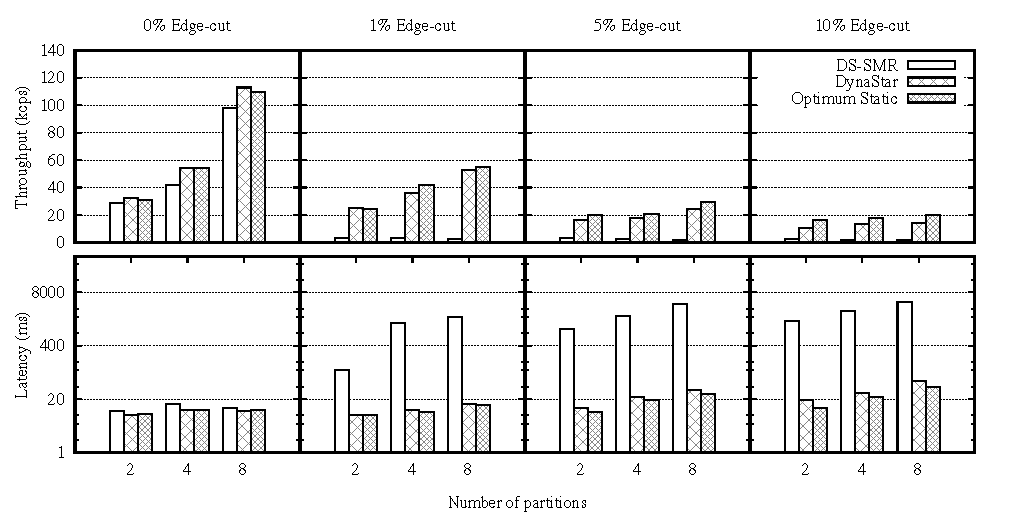
\includegraphics{figures/experiments/throughput-latency-avg-all}
	\caption{Throughput and latency, varying edge-cuts for different partitioning size}
	\label{fig:latency-avg-all}
\end{figure*}

The Figure~\ref{fig:move_throughput_ddsm_vs_dynastar} shows how a weak locality graph affects performance of \dssmr and \dynastar performance (i.e. centralized and decentralized methods). \dssmr couldn't reach a stable partitioning, and moved objects constantly, which prevents it from increasing performance. With \dynastar{}, it soon reach the optimal partitioning, help reducing the number of moves, and increasing the system's throughput

To test if the oracle can be a bottleneck, in Figure~\ref{fig:cpu_oracle} we show the average load over time in the oracle.
The load is higher in the beginning, when the clients did not yet cache the requests, but diminish over time, being
necessary only when clients have an invalid log or when a repartition happens.



\begin{figure*}[ht!]
  \centering
  \begin{subfigure}[b]{0.45\textwidth}
    \centering
    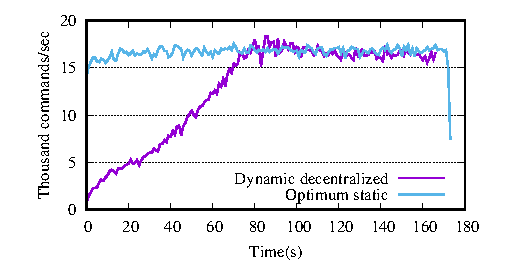
\includegraphics[width=0.95\columnwidth]{figures/motivation-tp-strong-locality}    
    \caption{Throughput with strong locality \lle{will be replaced}}
  \end{subfigure}
  \begin{subfigure}[b]{0.45\textwidth}
    \centering
    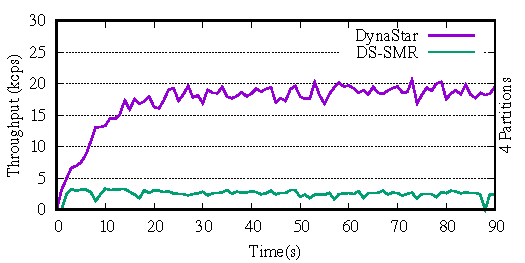
\includegraphics[width=0.95\columnwidth]{figures/experiments/tp-dynastar-vs-dssmr-4p}
    \caption{Throughput with weak locality}
  \end{subfigure} \\
  \begin{subfigure}[b]{0.45\textwidth}
    \centering
    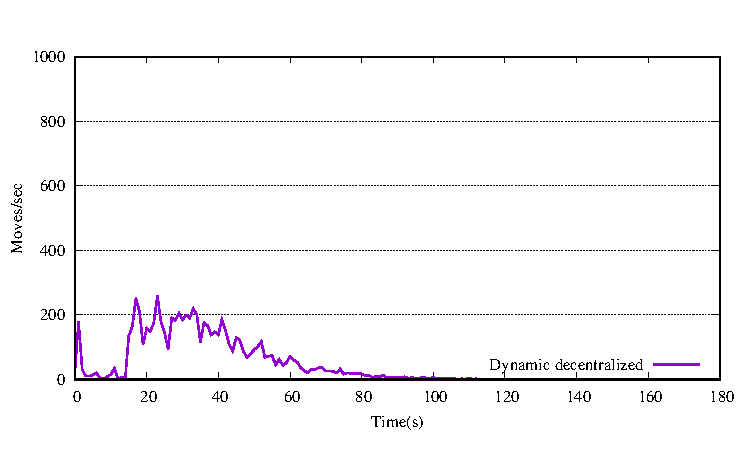
\includegraphics[width=0.95\columnwidth]{figures/motivation-moves-strong-locality}
    \caption{Number of move commands with strong locality \lle{will be replaced}}
  \end{subfigure}
  \begin{subfigure}[b]{0.45\textwidth}
    \centering
    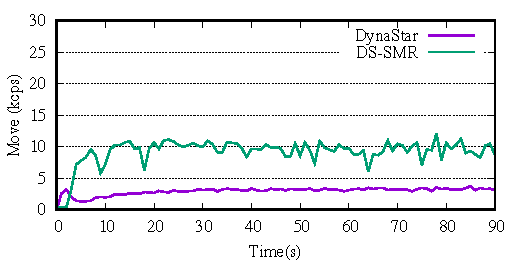
\includegraphics[width=0.95\columnwidth]{figures/experiments/move-dynastar-vs-dssmr-4p}
    \caption{Number of move commands with weak locality}
  \end{subfigure}
  \caption{Throughput and number of move commands for different level of locality}
  \label{fig:motivation}
\end{figure*}


\begin{figure}
\centering
\begin{subfigure}[ht]{0.5\textwidth}
\captionsetup{justification=centering}
	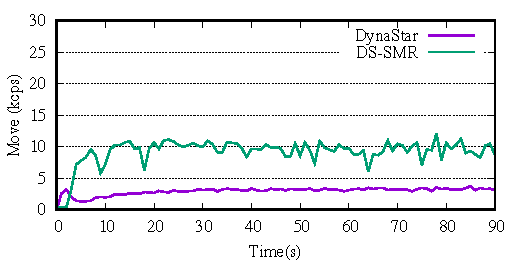
\includegraphics{figures/experiments/move-dynastar-vs-dssmr-4p}
	\caption{\dynastar and \dssmr\ moves over time}
	\label{fig:4p_moves}
\end{subfigure}

\begin{subfigure}[ht]{0.5\textwidth}
	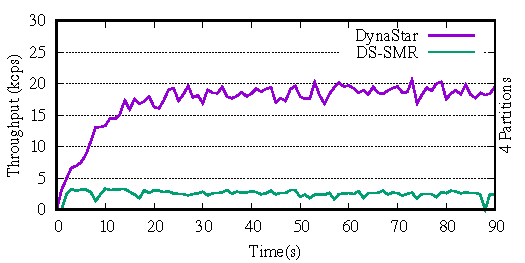
\includegraphics{figures/experiments/tp-dynastar-vs-dssmr-4p}
	\caption{\dynastar and \dssmr\ throughput over time}
	\label{fig:4p_tput}
\end{subfigure}
\label{fig:move_throughput_ddsm_vs_dynastar}
\end{figure}


We also verified if the oracle could be a bottleneck. in Figure~\ref{fig:cpu_oracle} we show the average load over time in the oracle.
The load is higher in the beginning, when the clients did not yet cache the requests, and \dynastar were trying to move objects to partitions as partitioning reference. After the partitioning had been better, the load on oracle become stable.

\begin{figure}[t]
	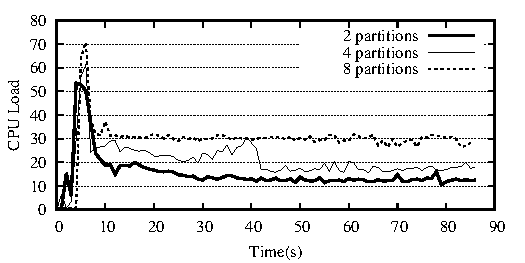
\includegraphics{figures/experiments/oracle-load}
	\caption{CPU load in the oracle}
	\label{fig:cpu_oracle}
\end{figure}

In Figure~\ref{fig:dynamic_load_tput}, we increase the number of clients and perform dynamic repartitionings,

Figure~\ref{fig:dynamic_load_tput} depicts the test of dynamic repartitioning on-the-fly. 
We started the system with an empty graph (i.e. there was no user in the system). 
Then clients continuously create users and links betweens users during the experiment (running follow command). 
The oracle monitored changed in the graph's structure, trigger repartitioning when the number of changes exceed a threshold. 
Each time the repartitioning took place, the partitioning became better, helps the throughput increase. 

\begin{figure}[ht]
	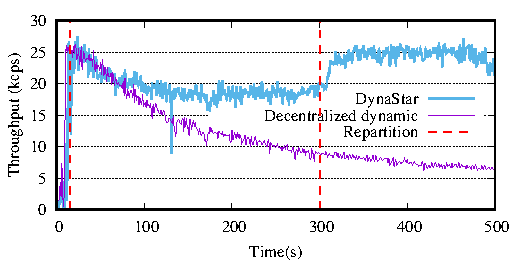
\includegraphics{figures/experiments/dynamicload-tp-move-4p}
	\caption{Adding nodes and repartitioning dynamically}
	\label{fig:dynamic_load_tput}
\end{figure}

\begin{figure}[ht]
	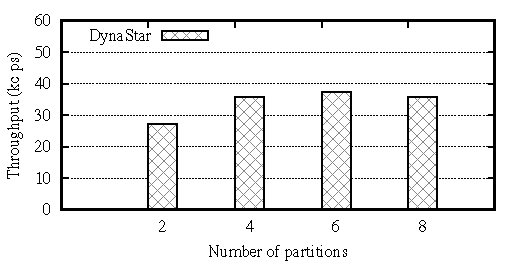
\includegraphics{figures/experiments/throughput-avg-vary-partition}
	\caption{Same graph in different partitioning}
	\label{fig:4p1p_varying_partition_size}
\end{figure}

\begin{figure}
\centering
\begin{subfigure}[ht]{0.5\textwidth}
\captionsetup{justification=centering}
	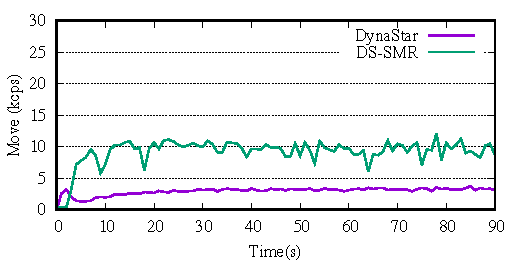
\includegraphics{figures/experiments/move-dynastar-vs-dssmr-4p}
	\caption{\dynastar and \dssmr\ moves over time}
	\label{fig:4p_moves}
\end{subfigure}

\begin{subfigure}[ht]{0.5\textwidth}
	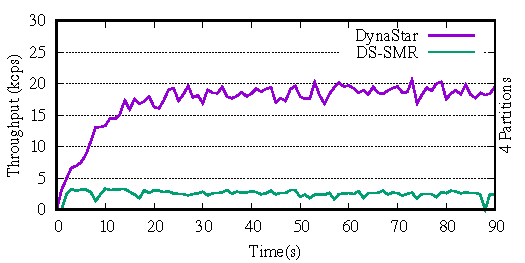
\includegraphics{figures/experiments/tp-dynastar-vs-dssmr-4p}
	\caption{\dynastar and \dssmr\ throughput over time}
	\label{fig:4p_tput}
\end{subfigure}
\end{figure}

\subsubsection{Dynamic partitioning}




\label{sec:evaluation:strongloc}

